
% This LaTeX was auto-generated from MATLAB code.
% To make changes, update the MATLAB code and republish this document.

\documentclass{article}
\usepackage{graphicx}
\usepackage{color}

\sloppy
\definecolor{lightgray}{gray}{0.5}
\setlength{\parindent}{0pt}

\begin{document}

    
    

\section*{26. Rational interpolation and linearized least-squares}

\begin{verbatim}
ATAPformats
\end{verbatim}
\begin{par}
For polynomials, we have emphasized that although best approximations with their equioscillating error curves are fascinating, Chebyshev interpolants or projections are just as good for most applications and simpler to compute since the problem is linear.  To some degree at least, the same is true of rational functions.  Best rational approximations are fascinating, but for practical purposes, it is often a better idea to use rational interpolants, and again an important part of the problem is linear since one can multiply through by the denominator.
\end{par} \vspace{1em}
\begin{par}
 But there is a big difference.  Rational interpolation problems
are not entirely linear, and unlike polynomial interpolation problems,
they suffer from both nonexistence and discontinuous dependence on data
in some settings. To use rational interpolants effectively, one must
formulate the problem in a way that minimizes such effects.  The method we
shall recommend for this, here and in the next two chapters, makes use of
the singular value decomposition (SVD) and the generalization of the
linearized interpolation problem to one of least-squares fitting. This
approach originates in [Pach\'on, Gonnet \& Van Deun 2012] and [Gonnet,
Pach\'on \& Trefethen 2011]. The literature of rational interpolation
goes back to Cauchy [1821] and Jacobi [1846], but much of it is rather
far from computational practice. 
\end{par} \vspace{1em}
\begin{par}
Here is an example to illustrate the difficulties. Suppose we seek a rational function $r\in {\cal R}_{11}$ satisfying the conditions $$ r(-1) = 2, \quad r(0) = 1, \quad r(1) = 2. \eqno (26.1) $$ Since a function in ${\cal R}_{11}$ is determined by three parameters, the count appears right for this problem to be solvable.   In fact, however, there is no solution, and one can prove this by showing that if a function in ${\cal R}_{11}$ takes equal values at two points, it must be a constant (Exercise 26.1). We conclude: solutions to seemingly sensible rational interpolation problems do not always exist.
\end{par} \vspace{1em}
\begin{par}
Let us modify the problem and seek a function $r\in {\cal R}_{11}$ satisfying the conditions $$ r(-1) = 1+\varepsilon, \quad r(0) = 1, \quad r(1) = 1+2\varepsilon, \eqno (26.2) $$ where $\varepsilon$ is a parameter. Now there is a solution for any $\varepsilon$, namely $$ r(z) = 1 + {{4\over 3}\varepsilon x\over x - {1\over 3}}. \eqno (26.3) $$ However, this is not quite the smooth interpolant one might have hoped for.  Here is the picture for $\varepsilon = 0.1$:
\end{par} \vspace{1em}
\begin{par}
 \vspace{-2em}
\end{par} \vspace{1em}
\begin{verbatim}
x = chebfun('x'); r = @(ep) 1 + (4/3)*ep*x./(x-(1/3));
ep = 0.1; hold off, plot(r(ep)), ylim([0 3])
hold on, plot([-1 0 1],[1+ep 1 1+2*ep],'.k')
FS = 'fontsize';
title('A type (1,1) rational interpolant through 3 data values',FS,9)
\end{verbatim}

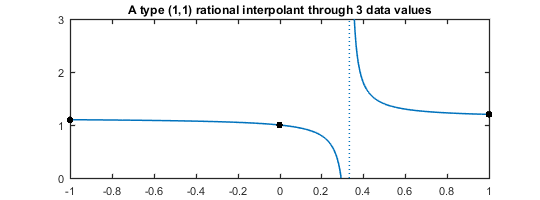
\includegraphics [width=4in]{chap26_01.png}
\begin{par}
 \vskip 1pt 
\end{par} \vspace{1em}
\begin{par}
And here it is for $\varepsilon = 0.001$:
\end{par} \vspace{1em}
\begin{par}
 \vspace{-2em} 
\end{par} \vspace{1em}
\begin{verbatim}
ep = 0.001; hold off, plot(r(ep)), ylim([0 3])
hold on, plot([-1 0 1],[1+ep 1 1+2*ep],'.k')
title('Same, with the data values now nearly equal',FS,9)
\end{verbatim}

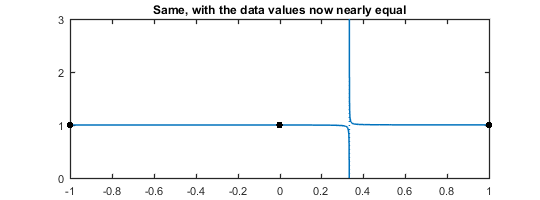
\includegraphics [width=4in]{chap26_02.png}
\begin{par}
 \vskip 1pt 
\end{par} \vspace{1em}
\begin{par}

Looking back at the formula (26.3), we see that for any nonzero value of
$\varepsilon$, this function has a pole at $x=1/3$.  When $\varepsilon$
is small, the effect of the pole is quite localized, and we may confirm
this by calculating that the residue is $(4/3)\varepsilon$.  Another way
to interpret the local effect of the pole is to note that $r$ has a zero
at a distance just $O(\varepsilon)$ from the pole:
$$ \hbox{pole: } x = \textstyle{1\over 3},  \qquad
   \hbox{zero: } x = \textstyle{1\over 3}/(1-\textstyle{4\over 3} \varepsilon). $$
For $|x-{1\over 3}|\gg \varepsilon$, the pole and the zero will
effectively cancel. This example shows that even when a rational
interpolation problem has a unique solution, the problem may be ill-posed
in the sense that the solution depends discontinuously on the data.  For
$\varepsilon=0$, (26.3) reduces to the constant $r=1$, whereas for any
nonzero $\varepsilon$ there is a pole, though it seems to have little to
do with approximating the data.  Such poles are often called {\em
spurious poles}. Since a spurious pole is typically associated with a
nearby zero that approximately cancels its effect further away, another
term is {\em Froissart doublet}, named after the physicist Marcel
Froissart [Froissart 1969].
We may also say that the function has a {\em spurious pole-zero pair}.

\end{par} \vspace{1em}
\begin{par}
Here is an example somewhat closer to practical approximation.  Consider the function $f(x) = \cos(e^x)$,
\end{par} \vspace{1em}
\begin{par}
 \vspace{-2em} 
\end{par} \vspace{1em}
\begin{verbatim}
f = cos(exp(x));
\end{verbatim}
\begin{par}

and suppose we want to construct rational interpolants of type $(n,n)$ to
$f$ based on samples at $2n+1$ Chebyshev points in $[-1,1]$. Chebfun has
a command {\tt ratinterp} that will do this, and here is a table of the
maximum errors obtained by {\tt ratinterp} for $n = 1,2,\dots, 6$:

\end{par} \vspace{1em}
\begin{par}
 \vspace{-2em}
\end{par} \vspace{1em}
\begin{verbatim}
disp('    (n,n)       Error ')
for n = 1:6
  [p,q] = ratinterp(f,n,n);
  err = norm(f-p./q,inf);
  fprintf('    (%1d,%1d)     %7.2e\n',n,n,err)
end
\end{verbatim}

        \color{lightgray} \begin{verbatim}    (n,n)       Error 
    (1,1)     2.46e-01
    (2,2)     7.32e-03
    (3,3)         Inf
    (4,4)     6.11e-06
    (5,5)     4.16e-07
    (6,6)     6.19e-09
\end{verbatim} \color{black}
    \begin{par}
We seem to have very fast convergence, but what has gone wrong with the type $(3,3)$ approximant?  A plot reveals that the problem is a spurious pole:
\end{par} \vspace{1em}
\begin{par}
 \vspace{-2em}
\end{par} \vspace{1em}
\begin{verbatim}
[p,q] = ratinterp(f,3,3);
hold off, plot(p./q), hold on
xx = chebpts(7); plot(xx,f(xx),'.k')
title(['Type (3,3) rational interpolant ' ...
       'to cos(e^x) in 7 Chebyshev points'],FS,9)
xlim([-1.001,1])
\end{verbatim}

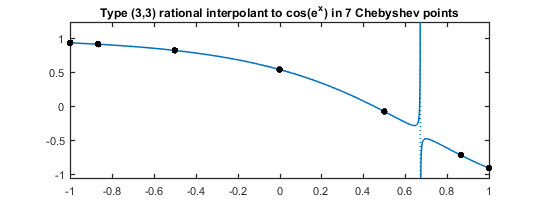
\includegraphics [width=4in]{chap26_03.png}
\begin{par}
 \vspace{1pt}
\end{par} \vspace{1em}
\begin{par}
One might suspect that this artifact has something to do with rounding errors on the computer, but it is not so. The spurious pole is in the mathematics, with residue equal to about $-0.0013$.
\end{par} \vspace{1em}
\begin{par}
 In other examples, on the other hand, spurious poles do indeed
arise from rounding errors.  In fact, they appear very commonly when one
aims for approximations with accuracy close to machine precision.  Here,
for example, is what happens when {\tt ratinterp} is called upon to
compute the interpolant of type $(8,8)$ of $e^x$ in $17$ Chebyshev
points:

\end{par} \vspace{1em}
\begin{par}
 \vspace{-2em}
\end{par} \vspace{1em}
\begin{verbatim}
[p,q] = ratinterp(exp(x),8,8,[],[],0);
hold off, plot(p./q), hold on
xx = chebpts(21); plot(xx,exp(xx),'.k','markersize',10)
title(['Type (8,8) interpolant to e^x, ' ...
       'not as good as it looks'],FS,9)
\end{verbatim}

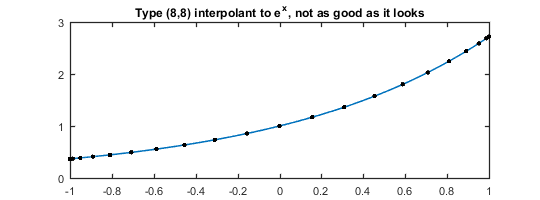
\includegraphics [width=4in]{chap26_04.png}
\begin{par}
 \vskip 1pt
\end{par} \vspace{1em}
\begin{par}
The picture looks fine, but that is only because Chebfun has failed to detect that $p/q$ has a spurious pole-zero pair:
\end{par} \vspace{1em}
\begin{par}
 \vspace{-2em}
\end{par} \vspace{1em}
\begin{verbatim}
spurious_zero = roots(p)
spurious_pole = roots(q)
\end{verbatim}

        \color{lightgray} \begin{verbatim}spurious_zero =
  -0.872966098101662
spurious_pole =
  -0.872966098101662
\end{verbatim} \color{black}
    \begin{par}
One could attempt to get around this particular pathology by computing in higher precision arithmetic.  However, quite apart from the practical difficulties of high-precision arithmetic, that approach would not really address the challenges of rational interpolation at a deeper level. The better response is to adjust the formulation of the rational interpolation problem so as to make it more robust. In this last example, it seems clear that a good algorithm should be sensible enough to reduce the number of computed poles. We now show how this can be done systematically with the SVD.
\end{par} \vspace{1em}
\begin{par}
At this point, we shall change settings.  Logically, we would now proceed to develop a robust rational interpolation strategy on $[-1,1]$. However, that route would require us to combine new ideas related to robustness with the complexities of Chebyshev points, Chebyshev polynomials, and rational barycentric interpolation formulas.  Instead, now and for most of the rest of the book, we shall move from the real interval $[-1,1]$ to the unit disk and switch variable names from $x$ to $z$. This will make the presentation simpler, and it fits with the fact that many applications of rational interpolants and approximants involve complex variables.
\end{par} \vspace{1em}
\begin{par}

Specifically, here is the problem addressed in the remainder of this
chapter, following [Pach\'on, Gonnet \& Van Deun 2012] and
[Gonnet, Pach\'on \& Trefethen 2011] but with roots as far back
as Jacobi [1846]. Suppose $f$ is a
function defined on the unit circle in the complex plane and we consider
its values $f(z_j)$ at the $(N+1)$st roots of unity for some $N\ge 0$,
$$ z_j = e^{2\pi ij/(N+1)}, \quad 0\le j \le N. $$
Using this information, how can we construct a good approximation $r\in
{\cal R}_{mn}$? We assume for the moment that $m$, $n$ and $N$ are related by
$N=m+n$.  The parameter count is then right for an interpolant $r = p/q$
satisfying
$$ {p(z_j)\over q(z_j)} = f(z_j), \quad 0\le j\le N. \eqno (26.4) $$
The problem of finding such a function $r$ is known as the
{\em Cauchy interpolation problem}.
As we have seen, however, a solution does not always exist.

\end{par} \vspace{1em}
\begin{par}

Our first step towards greater robustness will be to linearize the
problem and seek polynomials $p\in {\cal P}_m$ and $q\in {\cal P}_n$ such
that
$$ p(z_j) = f(z_j)\kern .7pt q(z_j), \quad 0\le j\le N. \eqno (26.5) $$
By itself, this set of equations isn't very useful, because it has the
trivial solution $p=q=0$.  Some kind of normalization is needed, and for
this we introduce the representations
$$ p(z) = \sum_{k=0}^m a_k z^k, \qquad  q(z) = \sum_{k=0}^n b_k z^k $$
with
$$ {\bf a} = (a_0,\dots, a_m)^T, \qquad {\kern .7pt\bf b} = (b_0,\dots, b_n)^T. $$
Our normalization will be the condition
$$\|{\kern .7pt\bf b}\| = 1, \eqno (26.6) $$
where $\|\cdot\|$ is the standard 2-norm on vectors,
$$ \|{\kern .7pt\bf b}\| = \left( \kern 2pt \sum_{k=0}^n |b_k|^2 \right)^{1/2}, $$
and similarly for vectors of dimensions other than $n+1$. Our linearized
rational interpolation problem consists of solving the two equations
(26.5)--(26.6).  A solution with $q(z_j)\ne 0$ for all $j$ will also satisfy
(26.4), but if $q(z_j)=0$ for some $j$, then (26.4) may or may not be
satisfied.  A point where it is not attained is called an
{\em unattainable point.}

\end{par} \vspace{1em}
\begin{par}

We turn (25.5)--(25.6) into a matrix problem as follows.
Given an arbitrary $(n+1)$-vector
${\kern .7pt\bf b}$, there is a corresponding polynomial $q\in {\cal P}_n$, which
we may evaluate at the $(N+1)$st roots of unity $\{z_j\}$. Multiplying by
the values $f(z_j)$ gives a set of $N+1$ numbers $f(z_j) q(z_j)$.  There
is a unique polynomial $\hat p\in {\cal P}_N$ that interpolates these
data,
$$ \hat p(z_j) = f(z_j) q(z_j), \quad 0 \le j \le N. $$
Let $\hat p$ be written as
$$ \hat p(z) = \sum_{k=0}^N \hat a_k z^k, \quad
{\bf \hat a} = (\hat a_0,\dots, \hat a_N)^T. $$ Then ${\bf \hat a}$ is a
linear function of ${\kern .7pt\bf b}$, and we may accordingly express it as the
product
$$ {\bf \hat a} = \hat C {\kern .7pt\bf b}, $$
where $\hat C$ is a rectangular matrix of dimensions $(N+1)\times (n+1)$
depending on $f$. It can be shown that $\hat C$ is a Toeplitz matrix with
entries given by the discrete Laurent or Fourier coefficients
$$ c_{jk} = {1\over N+1} \sum_{\ell=0}^N z_\ell^{k-j} f(z_\ell).
\eqno (26.7) $$
And now we can solve (26.5)--(26.6).  Let $\tilde C$ be the $n\times
(n+1)$ matrix consisting of the last $n$ rows of $\hat C$.  Since $\tilde
C$ has more columns than rows, it has a nontrivial null vector, and for
${\kern .7pt\bf b}$ we take any such null vector normalized to length $1$:
$$ \tilde C {\kern .7pt\bf b} = 0, \quad \|{\kern .7pt\bf b}\| = 1 . \eqno (26.8) $$
The corresponding vector ${\bf \hat a} = \hat C {\kern .7pt\bf b}$ is equal to zero
in positions $m+1$ through $N$, and we take ${\bf a}$ to be the
remaining, initial portion of ${\bf\hat a}$: $a_j=\hat a_j$, $0\le j\le
m$.  In matrix form we can write this as
$$ {\bf a} = C {\kern .7pt\bf b}, \eqno (26.9) $$
where $C$ is the $(m+1)\times (n+1)$ matrix consisting of the first
$m+1$ rows of $\hat C$.  Equations (26.8)--(26.9) constitute
a solution to (26.5)--(26.6).

\end{par} \vspace{1em}
\begin{par}
 In a numerical implementation of the algorithm just described,
the operations should properly be combined into a Matlab function, and
a function like this called {\tt ratdisk} is presented
in [Gonnet, Pach\'on \& Trefethen 2011].  Here, however,
for the sake of in-line presentation, we shall achieve the necessary
effect with a string of anonymous functions.

\end{par} \vspace{1em}
\begin{par}
The first step is to construct the Toeplitz matrix $\hat C$ using the Matlab \texttt{fft} command. The \texttt{real} command below eliminates imaginary parts at the level of rounding errors, and would need to be removed for a function $f$ that was not real on the real axis.
\end{par} \vspace{1em}
\begin{par}
 \vspace{-2em}
\end{par} \vspace{1em}
\begin{verbatim}
fj = @(f,N) f(exp(2i*pi*(0:N)'/(N+1)));
extract = @(A,I,J) A(I,J);
column = @(f,N) real(fft(fj(f,N)))/(N+1);
row = @(f,n,N) extract(column(f,N),[1 N+1:-1:N+2-n],1);
Chat = @(f,n,N) toeplitz(column(f,N),row(f,n,N));
\end{verbatim}
\begin{par}
Next we extract the submatrices $\tilde C$ and $C$:
\end{par} \vspace{1em}
\begin{par}
 \vspace{-2em}
\end{par} \vspace{1em}
\begin{verbatim}
Ctilde = @(f,m,n,N) extract(Chat(f,n,N),m+2:N+1,':');
C = @(f,m,n,N) extract(Chat(f,n,N),1:m+1,':');
\end{verbatim}
\begin{par}
Finally we compute the vector ${\kern .7pt\bf b}$ using the Matlab \texttt{null} command, which makes use of the SVD, and multiply by $C$ to get ${\bf a}$:
\end{par} \vspace{1em}
\begin{par}
 \vspace{-2em}
\end{par} \vspace{1em}
\begin{verbatim}
q = @(f,m,n,N) null(Ctilde(f,m,n,N));
p = @(f,m,n,N) C(f,m,n,N)*q(f,m,n,N);
\end{verbatim}
\begin{par}
For example, here are the coefficients of the type $(2,2)$ interpolant to $e^z$ in the 5th roots of unity:
\end{par} \vspace{1em}
\begin{par}
 \vspace{-2em}
\end{par} \vspace{1em}
\begin{verbatim}
f = @(z) exp(z); m = 2; n = 2; N = m+n;
pp = p(f,m,n,N), qq = q(f,m,n,N)
\end{verbatim}

        \color{lightgray} \begin{verbatim}pp =
  -0.893131422200046
  -0.446418130422149
  -0.074390723603151
qq =
  -0.891891822763679
   0.446093473426966
  -0.074361209330862
\end{verbatim} \color{black}
    \begin{par}
The zeros lie in the left half-plane and the poles in the right half-plane:
\end{par} \vspace{1em}
\begin{par}
 \vspace{-2em}
\end{par} \vspace{1em}
\begin{verbatim}
rzeros = roots(flipud(pp))
rpoles = roots(flipud(qq))
\end{verbatim}

        \color{lightgray} \begin{verbatim}rzeros =
 -3.000495954331881 + 1.732909565613550i
 -3.000495954331881 - 1.732909565613550i
rpoles =
  2.999503890813019 + 1.731191260767685i
  2.999503890813019 - 1.731191260767685i
\end{verbatim} \color{black}
    \begin{par}
Here are the values of the interpolant at $z=0$ and $z=2$, which one can see are not too far from $e^0$ and $e^2$:
\end{par} \vspace{1em}
\begin{par}
 \vspace{-2em}
\end{par} \vspace{1em}
\begin{verbatim}
r = @(z) polyval(flipud(pp),z)./polyval(flipud(qq),z);
approximation = r([0 2])
exact = exp([0 2])
\end{verbatim}

        \color{lightgray} \begin{verbatim}approximation =
   1.001389854021227   7.011719966971131
exact =
   1.000000000000000   7.389056098930650
\end{verbatim} \color{black}
    \begin{par}
Now let us take stock.  We have derived an algorithm for computing rational interpolants based on the linearized formula (26.5), but we have not yet dealt with spurious poles.  Indeed, the solution developed so far has neither uniqueness nor continuous dependence on data. It is time to take our second step toward greater robustness, again relying on the SVD.
\end{par} \vspace{1em}
\begin{par}
 An example will illustrate what needs to be done. Suppose that
instead of a type $(2,2)$ interpolant to $e^z$ in $5$ points, we want a
type $(8,8)$ interpolant in 17 points. (This is like the type $(8,8)$
interpolant computed earlier, but now in roots of unity rather than
Chebyshev points.) Here is what we find:

\end{par} \vspace{1em}
\begin{par}
 \vspace{-2em}
\end{par} \vspace{1em}
\begin{verbatim}
m = 8; n = 8; N = m+n;
format short
pp = p(f,m,n,N)
qq = q(f,m,n,N)
\end{verbatim}

        \color{lightgray} \begin{verbatim}pp =
   -0.1444   -0.9818
   -1.0168   -0.7969
   -0.4900   -0.2676
   -0.1118   -0.0517
   -0.0155   -0.0065
   -0.0014   -0.0006
   -0.0001   -0.0000
   -0.0000   -0.0000
   -0.0000   -0.0000
qq =
   -0.1444   -0.9818
   -0.8724    0.1849
    0.4546    0.0384
   -0.1062   -0.0189
    0.0148    0.0033
   -0.0013   -0.0003
    0.0001    0.0000
   -0.0000   -0.0000
    0.0000    0.0000
\end{verbatim} \color{black}
    \begin{par}
Instead of the expected vectors ${\bf a}$ and ${\kern .7pt\bf b}$, we have matrices of dimension $9\times 2$, and the reason is, $\tilde C$ has a nullspace of dimension 2.  This would not be true in exact arithmetic, but it is true in 16-digit floating-point arithmetic. If we construct an interpolant from one of these vectors, it will have a spurious pole-zero pair.  Here is an illustration, showing that the spurious pole (cross) and zero (circle) are near the unit circle, which is typical. The other seven non-spurious poles and zeros have moduli about ten times larger.
\end{par} \vspace{1em}
\begin{par}
 \vspace{-2em}
\end{par} \vspace{1em}
\begin{verbatim}
rpoles = roots(flipud(pp(:,1)));
rzeros = roots(flipud(qq(:,1)));
hold off, plot(exp(2i*pi*x))
ylim([-1.4 1.4]), axis equal, hold on
plot(rpoles,'xk','markersize',7)
plot(rzeros,'or','markersize',9)
title(['Spurious pole-zero pair in type ' ...
       '(10,10) interpolation of e^z'],FS,9)
\end{verbatim}

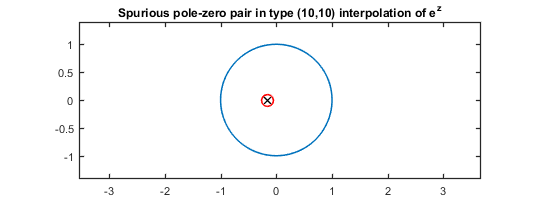
\includegraphics [width=4in]{chap26_05.png}
\begin{par}
 \vspace{1pt}
\end{par} \vspace{1em}
\begin{par}

Having identified the problem, we can fix it as follows. If $\tilde C$ has
rank $n-d$ for some $d\ge 1$, then it has a nullspace of dimension $d+1$.
(We intentionally use the same letter $d$ as was used to denote the
defect in Chapter 24.) There must exist a vector ${\kern .7pt\bf b}$ in this
nullspace whose final $d$ entries are zero.  We could do some linear
algebra to construct this vector, but a simpler approach is to reduce $m$
and $n$ by $d$ and $N$ by $2d$ and compute the interpolant again.  Here
is a function for computing $d$ with the help of the Matlab {\tt rank}
command, which is based on the SVD.\ \ The tolerance $10^{-12}$ ensures
that contributions close to machine precision are discarded.

\end{par} \vspace{1em}
\begin{par}
 \vspace{-2em}
\end{par} \vspace{1em}
\begin{verbatim}
d = @(f,m,n,N) n-rank(Ctilde(f,m,n,N),1e-12);
\end{verbatim}
\begin{par}
We redefine \texttt{q} and \texttt{p} to use this information:
\end{par} \vspace{1em}
\begin{par}
 \vspace{-2em}
\end{par} \vspace{1em}
\begin{verbatim}
q = @(f,m,n,N,d) null(Ctilde(f,m-d,n-d,N-2*d));
p = @(f,m,n,N,d) C(f,m-d,n-d,N-2*d)*q(f,m,n,N,d);
\end{verbatim}
\begin{par}
Our example now gives vectors instead of matrices, with no spurious poles.
\end{par} \vspace{1em}
\begin{par}
 \vspace{-2em}
\end{par} \vspace{1em}
\begin{verbatim}
pp = p(f,m,n,N,d(f,m,n,N)); qq = q(f,m,n,N,d(f,m,n,N));
format long
disp('           pp                  qq'), disp([pp qq])
\end{verbatim}

        \color{lightgray} \begin{verbatim}           pp                  qq
  -0.889761508658415  -0.889761508658261
  -0.444881277405721   0.444880231252617
  -0.101109524475056  -0.101109001398522
  -0.013481293405081   0.013481177143514
  -0.001123443581972  -0.001123429040899
  -0.000056172339474   0.000056171299382
  -0.000001337441849  -0.000001337407064
\end{verbatim} \color{black}
    \begin{par}
This type $(7,7)$ rational function approximates $e^z$ to approximately machine precision in the unit disk.  To verify this loosely, we write a function \texttt{error} that measures the maximum of $|f(z)-r(z)|$ over $1000$ random points in the disk:
\end{par} \vspace{1em}
\begin{par}
 \vspace{-2em}
\end{par} \vspace{1em}
\begin{verbatim}
r = @(z) polyval(flipud(pp),z)./polyval(flipud(qq),z);
z = sqrt(rand(1000,1)).*exp(2i*pi*rand(1000,1));
error = @(f,r) norm(f(z)-r(z),inf);
error(f,r)
\end{verbatim}

        \color{lightgray} \begin{verbatim}ans =
     8.482339972561138e-13
\end{verbatim} \color{black}
    \begin{par}

Mathematically, in exact arithmetic, the trick of reducing $m$ and $n$ by
$d$ restores uniqueness and continuous dependence on data, making the
rational interpolation problem well-posed.  On a computer, we do the same
but rely on finite tolerances to remove contributions from singular
values close to machine epsilon.  A much more careful version of this
algorithm can be found in the Matlab code {\tt ratdisk} from
[Gonnet, Pach\'on \& Trefethen 2011], mentioned earlier.

\end{par} \vspace{1em}
\begin{par}

We conclude this chapter by taking a third step towards robustness. So
far, we have spoken only of interpolation, where the number of data
values exactly matches the number of parameters in the fit. In some
approximation problems, however, it may be better to have more data than
parameters and perform a least-squares fit.  This is one of those
situations, and in particular, a least-squares formulation will reduce
the likelihood of obtaining poles in the region near the unit circle
where one is hoping for good approximation.  This is why we have included
the parameter $N$ throughout the derivation of the last six pages. We
will now consider the situation $N>m+n$. Typical choices for practical
applications might be $N = 2(m+n)$ or $N=4(m+n)$.

\end{par} \vspace{1em}
\begin{par}
Given an $(n+1)$-vector ${\kern .7pt\bf b}$ and corresponding function $q$, we have already defined $\|{\kern .7pt\bf b}\|$ as the usual 2-norm.  For the function $q$, let us now define $$ \|\kern .7pt q\|_N^{} = (N+1)^{-1/2} \sum_{k=0}^N |q(z_j)|^2 , $$ a weighted 2-norm of the values of $q(z)$ over the unit circle. So long as $N\ge n$, the two norms are equal: $$ \|q\|_N = \|{\kern .7pt\bf b}\|. $$ The norm $\|\cdot\|_N$, however, applies to any function, not just a polynomial.  In particular, our linearized least-squares rational approximation problem is this generalization of (26.5)--(26.6): $$ \|\kern .7pt p-fq\|_N = \hbox{minimum}, \quad \|q\|_N = 1. \eqno (26.10) $$ The algorithm we have derived for interpolation solves this problem too. What changes is that the matrix $\tilde C$, of dimension $(N-m)\times (n+1)$, may no longer have a null vector. If its singular values are $\sigma_1 \ge \cdots \ge \sigma_{n+1} \ge 0$, then the minimum error will be $$ \|\kern .7pt p-fq\|_N = \sigma_{n+1}, $$ which may be positive or zero.  If $\sigma_n>\sigma_{n+1}$, ${\kern .7pt\bf b}$ is obtained from the corresponding singular vector and that is all there is to it.  If $$ \sigma_{n-d} > \sigma_{n-d+1} = \cdots = \sigma_{n+1} $$ for some $d\ge 1$, then the minimum singular space is of dimension $d+1$, and as before, we reduce $m$ and $n$ by $d$. The parameter $N$ can be left unchanged, so $f$ does not need to be evaluated at any new points.
\end{par} \vspace{1em}
\begin{par}
For example, let $f$ be the function $f(z) = \log(1.44-z^2)$,
\end{par} \vspace{1em}
\begin{par}
 \vspace{-2em}
\end{par} \vspace{1em}
\begin{verbatim}
f = @(z) log(1.44-z.^2);
\end{verbatim}
\begin{par}
with branch points at $\pm 1.2$, and suppose we want a type $(40,40)$ least-squares approximant with $N=400$.  The approximation delivered by the SVD algorithm comes out with exact type $(18,18)$:
\end{par} \vspace{1em}
\begin{par}
 \vspace{-2em}
\end{par} \vspace{1em}
\begin{verbatim}
m = 40; n = 40; N = 400;
pp = p(f,m,n,N,d(f,m,n,N)); qq = q(f,m,n,N,d(f,m,n,N));
mu = length(pp)-1; nu = length(qq)-1;
fprintf('    mu = %2d    nu = %2d\n',mu,nu)
\end{verbatim}

        \color{lightgray} \begin{verbatim}    mu = 18    nu = 18
\end{verbatim} \color{black}
    \begin{par}
The accuracy in the unit disk is good (Exercise 26.4):
\end{par} \vspace{1em}
\begin{par}
 \vspace{-2em}
\end{par} \vspace{1em}
\begin{verbatim}
r = @(z) polyval(flipud(pp),z)./polyval(flipud(qq),z);
error(f,r)
\end{verbatim}

        \color{lightgray} \begin{verbatim}ans =
     7.074122695603229e-12
\end{verbatim} \color{black}
    \begin{par}
Here are the poles:
\end{par} \vspace{1em}
\begin{par}
 \vspace{-2em}
\end{par} \vspace{1em}
\begin{verbatim}
rpoles = roots(flipud(qq));
hold off, plot(exp(2i*pi*x))
ylim([-1.4 1.4]), axis equal, hold on
plot(rpoles+1e-10i,'.r','markersize',14)
title(['Poles in type (40,40) robust ' ...
       'approximation of log(1.44-z^2)'],FS,9)
\end{verbatim}

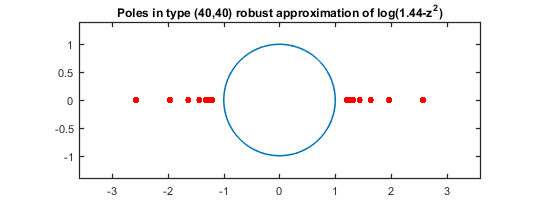
\includegraphics [width=4in]{chap26_06.png}
\begin{par}
 \vspace{1pt}
\end{par} \vspace{1em}
\begin{par}

For comparison, suppose we revert to the original definitions of the
anonymous functions {\tt p} and {\tt q}, with no removal of negligible
singular values:

\end{par} \vspace{1em}
\begin{par}
 \vspace{-2em}
\end{par} \vspace{1em}
\begin{verbatim}
q = @(f,m,n,N) null(Ctilde(f,m,n,N));
p = @(f,m,n,N) C(f,m,n,N)*q(f,m,n,N);
\end{verbatim}
\begin{par}
Now the computation comes out with exact type $(40,40)$, and half the poles are spurious:
\end{par} \vspace{1em}
\begin{par}
 \vspace{-2em}
\end{par} \vspace{1em}
\begin{verbatim}
m = 40; n = 40; N = 400;
pp = p(f,m,n,N); pp = pp(:,end);
qq = q(f,m,n,N); qq = qq(:,end);
rpoles = roots(flipud(qq));
hold off, plot(exp(2i*pi*x))
ylim([-1.4 1.4]), axis equal, hold on
plot(rpoles+1e-10i,'.r','markersize',14)
title(['The same computed without robustness, ' ...
       'showing many spurious poles'],FS,9)
\end{verbatim}

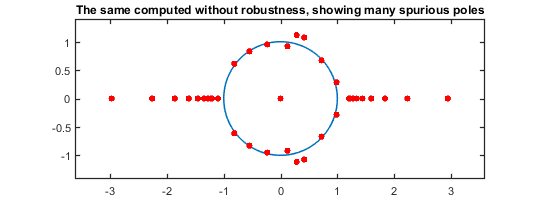
\includegraphics [width=4in]{chap26_07.png}
\begin{par}
 \vspace{1pt}
\end{par} \vspace{1em}
\begin{par}
The error looks excellent,
\end{par} \vspace{1em}
\begin{par}
 \vspace{-2em}
\end{par} \vspace{1em}
\begin{verbatim}
r = @(z) polyval(flipud(pp),z)./polyval(flipud(qq),z);
error(f,r)
\end{verbatim}

        \color{lightgray} \begin{verbatim}ans =
     3.492927538587022e-14
\end{verbatim} \color{black}
    \begin{par}
but in fact it is not so good.  Because of the spurious poles, the maximum error in the unit disk is actually infinite, but this has gone undetected at the 1000 random sample points used by the \texttt{error} command.
\end{par} \vspace{1em}
\begin{par}
In closing this chapter we return for a moment to the variable $x$ on the interval $[-1,1]$.  Earlier we used the Chebfun command \texttt{ratinterp} to compute a type $(8,8)$ interpolant to $e^x$ in Chebyshev points and found that it had a spurious pole-zero pair introduced by rounding errors.  This computation was one of pure interpolation, with no SVD-related safeguards of the kind described in the last few pages.  However, \texttt{ratinterp} is actually designed to incorporate SVD robustness by default.  The earlier computation called \texttt{ratinterp(exp(x),8,8,[],[],0)} in order to force a certain SVD tolerance to be $0$ instead of the default $10^{-14}$. If we repeat the computation with the default robustness turned on, we find that an approximation of exact type $(8,4)$ is returned and it has no spurious pole and zero:
\end{par} \vspace{1em}
\begin{verbatim}
[p,q,rh,mu,nu] = ratinterp(exp(x),8,8);
mu, nu
spurious_zero = roots(p)
spurious_pole = roots(q)
\end{verbatim}

        \color{lightgray} \begin{verbatim}mu =
     8
nu =
     4
spurious_zero =
   Empty matrix: 0-by-1
spurious_pole =
   Empty matrix: 0-by-1
\end{verbatim} \color{black}
    \begin{par}

\begin{displaymath}
\framebox[4.7in][c]{\parbox{4.5in}{\vspace{2pt}\sl
{\sc Summary of Chapter 26.}  Generically, there exists a unique type
$(m,n)$ rational interpolant through $m+n+1$ data points, but such
interpolants do not always exist, depend discontinuously on the data, and
exhibit spurious pole-zero pairs both in exact arithmetic and even more
commonly in floating point.  They can be computed by solving
a matrix problem involving a Toeplitz matrix of discrete Fourier
coefficients.  Uniqueness, continuous dependence, and avoidance of
spurious poles can be achieved by reducing $m$ and $n$ when the minimal
singular value of this matrix is multiple.  It may also be helpful to
oversample and solve a least-squares problem. \vspace{2pt}}}
\end{displaymath}

\end{par} \vspace{1em}
\begin{par}
\small
\parskip=2pt
\par
{\bf Exercise 26.1.  Nonexistence of certain interpolants.}
Show that if a function in ${\cal R}_{11}$ takes equal values at two points,
it must be a constant.
\par
{\bf Exercise 26.2.  An invalid argument.}  We saw that the type $(3,3)$
interpolant to $\cos(e^x)$ in 7 Chebyshev points has a pole near $x=0.6$.
What is the flaw in the following argument?  (Spell it out carefully,
don't just give a word or two.)  The interpolant through these 7 data
values can be regarded as a combination of cardinal functions, i.e., type
$(3,3)$ rational interpolants through Kronecker delta functions supported
at each of the data points.  If the sum has a pole at $x_0$, then one of
the cardinal interpolants must have a pole at $x_0$.  So type $(3,3)$
rational interpolants to almost every set of data at these 7 points will
have a pole at exactly the same place.
\par
{\bf Exercise 26.3.  Explicit example of degeneracy.}  Following the
example (26.2)--(26.3), but now on the unit circle, let $r$ be the
type $(1,1)$ rational function satisfying $r(1) = 1$, $r(\omega) = 1+i\kern .5pt\varepsilon$,
$r(\overline\omega) = 1-i\kern .5pt\varepsilon$, where $\omega$ is the cube root of $1$ in
the upper half-plane and $\varepsilon>0$ is a parameter.
(a) What is $r$?
(b) What is the $2\times 3$ matrix $\hat C$ of (26.7)?
(c) How do the singular values of $\hat C$ behave as $\varepsilon\to 0\kern .7pt$?
\par
{\bf Exercise 26.4.  Rational vs.\ polynomial approximation.} The final
computational example of this chapter considered type $(n,n)$ rational
approximation of $f(z) = \log(1.44-z^2)$ with $n=40$, which was reduced
to $n=18$ by the robust algorithm.  For degree $2n$ polynomial
approximation, one would expect accuracy of order $O(\rho^{-2n})$ where
$\rho$ is the radius of convergence of the Taylor series of $f$ at $z=0$.
How large would $n$ need to be for this figure to be comparable to the
observed accuracy of $10^{-11}\kern .7pt $?
\par
{\bf Exercise 26.5.  Rational Gibbs phenomenon} (from [Pach\'on 2010, Sec.~5.1]).
We saw in Chapter 9
that if $f(x) = \hbox{sign}(x)$ is interpolated by polynomials in Chebyshev
points in $[-1,1]$, the errors decay inverse-linearly with distance from the
discontinuity.  Use {\tt ratinterp} to explore the analogous rates of
decay for type $(m,2)$ and $(m,4)$ linearized rational interpolants to
the same function, keeping $m$ odd for simplicity.  What do the decay rates appear to be?
\par
{\bf Exercise 26.6.  A function with two rows of poles.}
After Theorem 22.1 we considered as an example the function
$f(x) = (2+\cos(20x+1))^{-1}$.  (a) Call {\tt ratinterp}
with $(m,n) = (100,20)$ to determine a rational approximation $r$ to $f$
on $[-1,1]$ with up to $20$ poles.  How many poles does $r$ in fact have, and
what are they?
(b) Determine analytically the full set of poles of $f$ and produce a plot
of the approximations from (a) together with the nearby poles of $f$.  How accurate
are these approximations?

\end{par} \vspace{1em}



\end{document}
    
